\documentclass[bibliography=totoc]{scrartcl}
\usepackage[ngerman, english]{babel}
\usepackage{rwukoma}
\usepackage[pdfusetitle]{hyperref}
\usepackage{lipsum,caption}
\usepackage{algorithm, algpseudocode}
\usepackage{graphicx}
\usepackage{subcaption}
\usepackage{float}
\usepackage{amsmath}
\usepackage{pythonhighlight}

\setlength{\belowcaptionskip}{5pt}

\title{Camera Calibration}
\author{Leopold Gaube - 34948, IN}
\date{\today}

\begin{document}
\maketitle
\tableofcontents

\clearpage

\section{Task Overview}

When taking images or video with a camera, a 3D scene gets projected onto a 2D image.
A simple pinhole camera model is still often used explain the concept of this projection, but nowadays modern cameras use lenses to capture more light.
This gives rise to a problem where supposed straight lines, for instance a door, do appear curved in the resulting image. 
This unwanted effect is called lens distortion and is usually most pronounced with ultrawide lenses.

The following report presents an algorithm to calibrate a camera and undistort images based on this calibration.
Two calibration videos, each depicting a checkerboard pattern in various positions, has been provided by the lecturer of the Computer Vision course.
In both videos Barrel Distortion is clearly visible and its removal is the objective of the hereby presented algorithm.

First, the algorithm extracts appropriate frames from the calibration video.
Then in each calibration frame the checkerboard pattern is localized.
These positions are used to retrieve the intrinsic matrix and distortion coefficients of the camera. 
Together they allow to undistort any image taken with the same camera, which is finally demonstrated on the calibration frames themselves.

The code and all frames used for the camera calibration task are available in this \href{https://gitlab.com/gaubeleo/camera-calibration}{GitLab repository} \cite{Gitlab}.

\section{Frame Selection}
In theory, we only need three frames to retrieve the intrinsic camera matrix. (why?)
In practise, more frames give better results and it is also advisable to use frames with the checkerboard present in different parts of the image and with varying distance.
The OpenCV documentation advises to use at least ten images for a camera calibration \cite{CameraCalibration}.
It is possible to manually extract appropriate frames from the calibration video, but we chose to automate this process in order to minimize work for the user in future calibrations. 

Naturally, consecutive frames should not be used, but frames that span the entire video.
For this, the video gets sectioned into 20 evenly spaced time steps and we try to find an appropriate frame for each section.
This way, we get varying checkerboard positions, assuming the checkerboard is being moved around in the calibration video.

Some of the frames may have a lot of motion blur which can be problematic for accurately localizing the checkerboard corners.
Instead of choosing calibration frames in fixed intervals, we consider 25 consecutive candidate frames for each video section (corresponding to one second of video) from which we only choose the least blurred one. (ToDo: Grafik?)
The extent of blur in an image can be calculated using the Variance of Laplacian, with a low variance corresponding to a high amount of blur \cite{BlurDetection}.
With OpenCV it is simple to obtain a focus measure for any greyscale image:

\begin{python}
    focus_score = cv2.Laplacian(frame, cv2.CV_64F).var()
\end{python}

The absolute value is of no interest, but the highest value of the 25 candidate frames corresponds to the sharpest one.


\section{Intrinsic Camera Matrix}
The intrinsic matrix is defined as

$$
K =
\begin{pmatrix}
    f_x & 0 & c_x \\
    0 & f_y & c_x \\
    0 & 0 & 1
\end{pmatrix}
$$

with $f_x$, $f_y$ representing the focal length and $c_x$, $c_y$ representing the optical center in x and y direction, respectively \cite{CameraCalibration}.
Together with the distortion coefficients 

$$(k_1, k_2, p_1, p_2, k_3)$$

the intrinsic matrix can be used to undistort images.

K is an upper triangular matrix, therefore, the determinant of K is the product of its trace, 
which is non-zero because the focal lengths $f_x$ and $f_y$ are always greater than 0. 

In order to estimate the instrinsic camera matrix and distortion coefficients, a predefined object has to be detected and localized in the calibration frames.
This algorithm uses a checkerboard as such a predefined object, because it possesses adventagious properties that simplify the calibration process.
Because a checkerboard is flat, all detection points lay on the same plane in equal distance to each other.
Both calibration videos show a board with 8x8 squares, but only corner points of four intersecting squares are used, thus, it depicts a 7x7 pattern.

Unfortunately, even with sharp images it is not guaranteed that OpenCV can always locate the checkerboard.
Successful detections are highly dependant on the size of the pattern. 
Curiously, the 7x7 pattern is rarly detected even when the full checkerboard is clearly visible in the image frame.
Smaller patterns are detected more frequently.
The 6x6 pattern is recognised in some checkerboard positions, but not in others, so a 5x5 pattern is chosen for this algorithm.
Using the adaptiveThreshold and normalizeImage flags also improves the detection consistency.
In both videos, the 5x5 checkerboard pattern can be found in 13 of the 20 sections, which fulfills the OpenCV recommendation of at least ten images.

The cv2.findChessboard() method only localizes the checkerboard pattern in terms of pixel coordinates, which is inprecise.
With cv2.cornerSubPix() these coordinates can be refined to sub-pixel precision.

In addition to the 2D image positions of all detected checkerboards, the corresponding 3D real-world object positions are also needed.
The world coordinate system can be set to any position. 
Canonically, we choose the left top corner of the checkerboard as its origin.
Furthermore, the distance between each checkerboard square is set to be one unit in both x and y direction. 
The checkerboard is flat, which allows all object points to sit on the z=0 plane.
This makes it possible to set identical real-world object positions for all 15 calibration frames.

\begin{figure}[ht!]
	\centering
	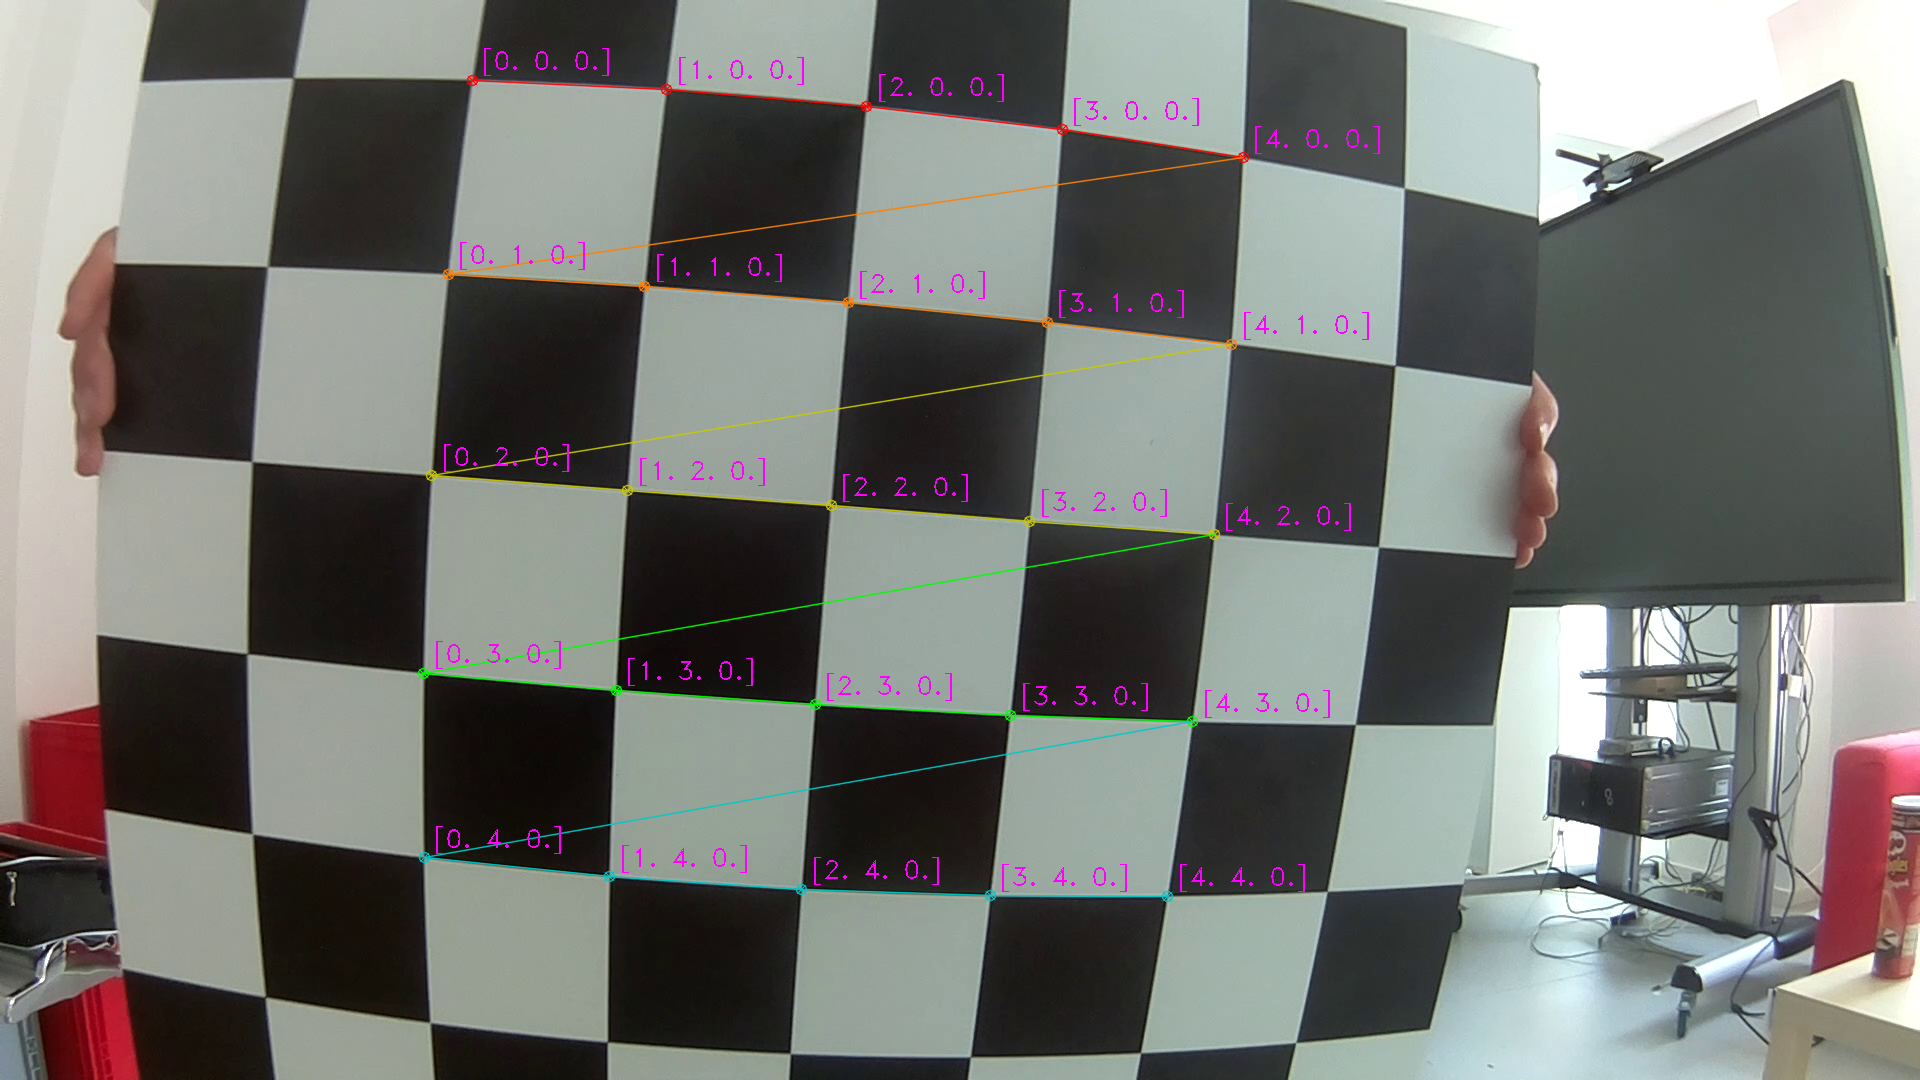
\includegraphics[width=\linewidth]{imgs/labeled_checkerboard.png}
	\caption{The detected checkerboard corners overlayed with its corresponding object point positions.}
	\label{fig:labeled_checkerboard}
\end{figure}


\section{Results}
OpenCV provides a functionality to calculate the intrinsic camera matrix and distortion coefficients automatically from the object positions and corresponding image positions.
In addition, it also provides rotation and translation vectors.
These are not required for undistorting images, but will later be used for projecting the object points onto the image in order to calculate the calibration error.

\begin{python}
ret, int_mtx, dist_coef, rot_vecs, trans_vecs = cv.calibrateCamera(
    world_points_3d, img_points_2d, (1920, 1080), None, None
)
\end{python}

undistort...!

Undistorting images result in some black regions on the edges where there is no information in the orignal image.
We crop these regions to obtain clean undistorted images.

In order to measure the quality of the calibration, the 3D real-world object points can be projected back onto to 2D image points using the intrinsic matrix and distortion coefficients as well as the rotational and translational vectors.
The closer they are to the detected checkerboard corners the smaller the reprojection error and the better the calibration.

Our Algorithm retrieved the following intrinsic matrix for the old video

$$
K =
\begin{pmatrix}
    2157.65015388 & 0. & 993.94771538 \\
    0. & 2189.00413434 & 511.18730768 \\
    0. & 0. & 1.
\end{pmatrix}
$$

with distortion coefficients

$$(-0.83698399, 0.69455783, -0.01109099, -0.01136698, 0.0078521)$$

and a mean reprojection error of 0.09529720894585678.

For the new video it produced 

$$
K =
\begin{pmatrix}
    2157.65015388 & 0. & 993.94771538 \\
    0. & 2189.00413434 & 511.18730768 \\
    0. & 0. & 1.
\end{pmatrix}
$$

with distortion coefficients

$$(-0.83698399, 0.69455783, -0.01109099, -0.01136698, 0.0078521)$$

and a mean reprojection error of 0.09529720894585678.

The intrinsic matrices gets saved to a file, as it has to be calculated only once and can be reused to undistort images taken in different scenes assuming the same camera is being used.

\clearpage
\bibliographystyle{alpha}
\bibliography{literature}
\end{document}
